\section{Appendix}

\subsection{Repository Structure}

\begin{verbatim}
chicago-crimes-pipeline/
|-- main.sh                          # Master orchestrator
|-- README.md                        # Project documentation
|-- data/
|   |-- chicago_crimes_raw.csv       # Raw CSV download
|   |-- train.json                   # Training split
|   |-- test.json                    # Test split
|-- scripts/
|   |-- data_collection.sh           # Socrata API download
|   |-- build_db.py                  # PostgreSQL database creation
|   |-- sqoop_import.sh              # Sqoop import with benchmarks
|   |-- eda_pyspark.py               # 7 EDA queries
|   |-- ml_pipeline.py               # Full ML pipeline
|   |-- load_postgres.py             # PostgreSQL loader for ML results
|   |-- stage2.sh                    # Stage II orchestrator
|   |-- stage3.sh                    # Stage III orchestrator
|   |-- stage4.sh                    # Stage IV orchestrator
|   |-- verify.sh                    # Data integrity checks
|-- sql/
|   |-- hive_create.sql             # Hive DDL
|   |-- db.hql                       # Hive optimizations
|-- output/
|   |-- q1.csv ... q7.csv           # EDA query results
|   |-- q1.jpg ... q7.jpg           # EDA chart exports
|   |-- dashboard.jpg               # Stage II dashboard
|   |-- dashboard_stage4.jpg        # Stage IV dashboard
|   |-- evaluation.csv              # Model comparison
|   |-- model1_predictions.csv      # RF predictions
|   |-- model2_predictions.csv      # GBT predictions
|-- models/
|   |-- model1/                     # Saved RF model
|   |-- model2/                     # Saved GBT model
|-- docs/
|   |-- MS_Stage1_Report.md         # Stage I report
|   |-- MS_Stage2_Report.md         # Stage II report
|   |-- MS_Stage3_Report.md         # Stage III report
|   |-- MS_Stage4_Report.md         # Stage IV report
|   |-- superset_instructions.md    # Superset setup guide
|-- base/
|   |-- packages.tex                # LaTeX packages
|   |-- style.tex                   # LaTeX style
|-- sections/
|   |-- *.tex                       # Report sections
|-- report.tex                      # Main LaTeX document
|-- bibliography.bib                # References
\end{verbatim}

\subsection{Cluster Access Information}

\begin{itemize}
    \item \textbf{Cluster}: IU Hadoop cluster (\texttt{hadoop-01.uni.innopolis.ru})
    \item \textbf{User}: \texttt{team2}
    \item \textbf{HiveServer2}: \texttt{hadoop-03.uni.innopolis.ru:10001}
    \item \textbf{PostgreSQL}: \texttt{hadoop-04.uni.innopolis.ru:5432}
    \item \textbf{Superset}: \texttt{http://hadoop-03.uni.innopolis.ru:8808}
    \item \textbf{Main script}: \texttt{/home/team2/project/main.sh}
\end{itemize}

\subsection{Sqoop Command}

\begin{lstlisting}[language=bash, caption={Sqoop import command}]
sqoop import \
    --connect jdbc:postgresql://hadoop-04.uni.innopolis.ru:5432/team2_projectdb \
    --username team2 --password V2P1hy6zjPqWoXMm \
    --table crimes \
    --split-by id \
    --num-mappers 4 \
    --as-parquetfile \
    --compress --compression-codec org.apache.hadoop.io.compress.SnappyCodec \
    --target-dir /user/team2/project/warehouse/crimes
\end{lstlisting}

\subsection{Spark Submit Command}

\begin{lstlisting}[language=bash, caption={Spark ML pipeline submission}]
spark-submit \
    --master yarn \
    --deploy-mode cluster \
    --num-executors 4 \
    --executor-memory 4g \
    --executor-cores 2 \
    --driver-memory 4g \
    scripts/ml_pipeline.py
\end{lstlisting}

\subsection{Dashboard Screenshots}

\subsubsection{Stage IV Superset Dashboard}

\begin{figure}[H]
    \centering
    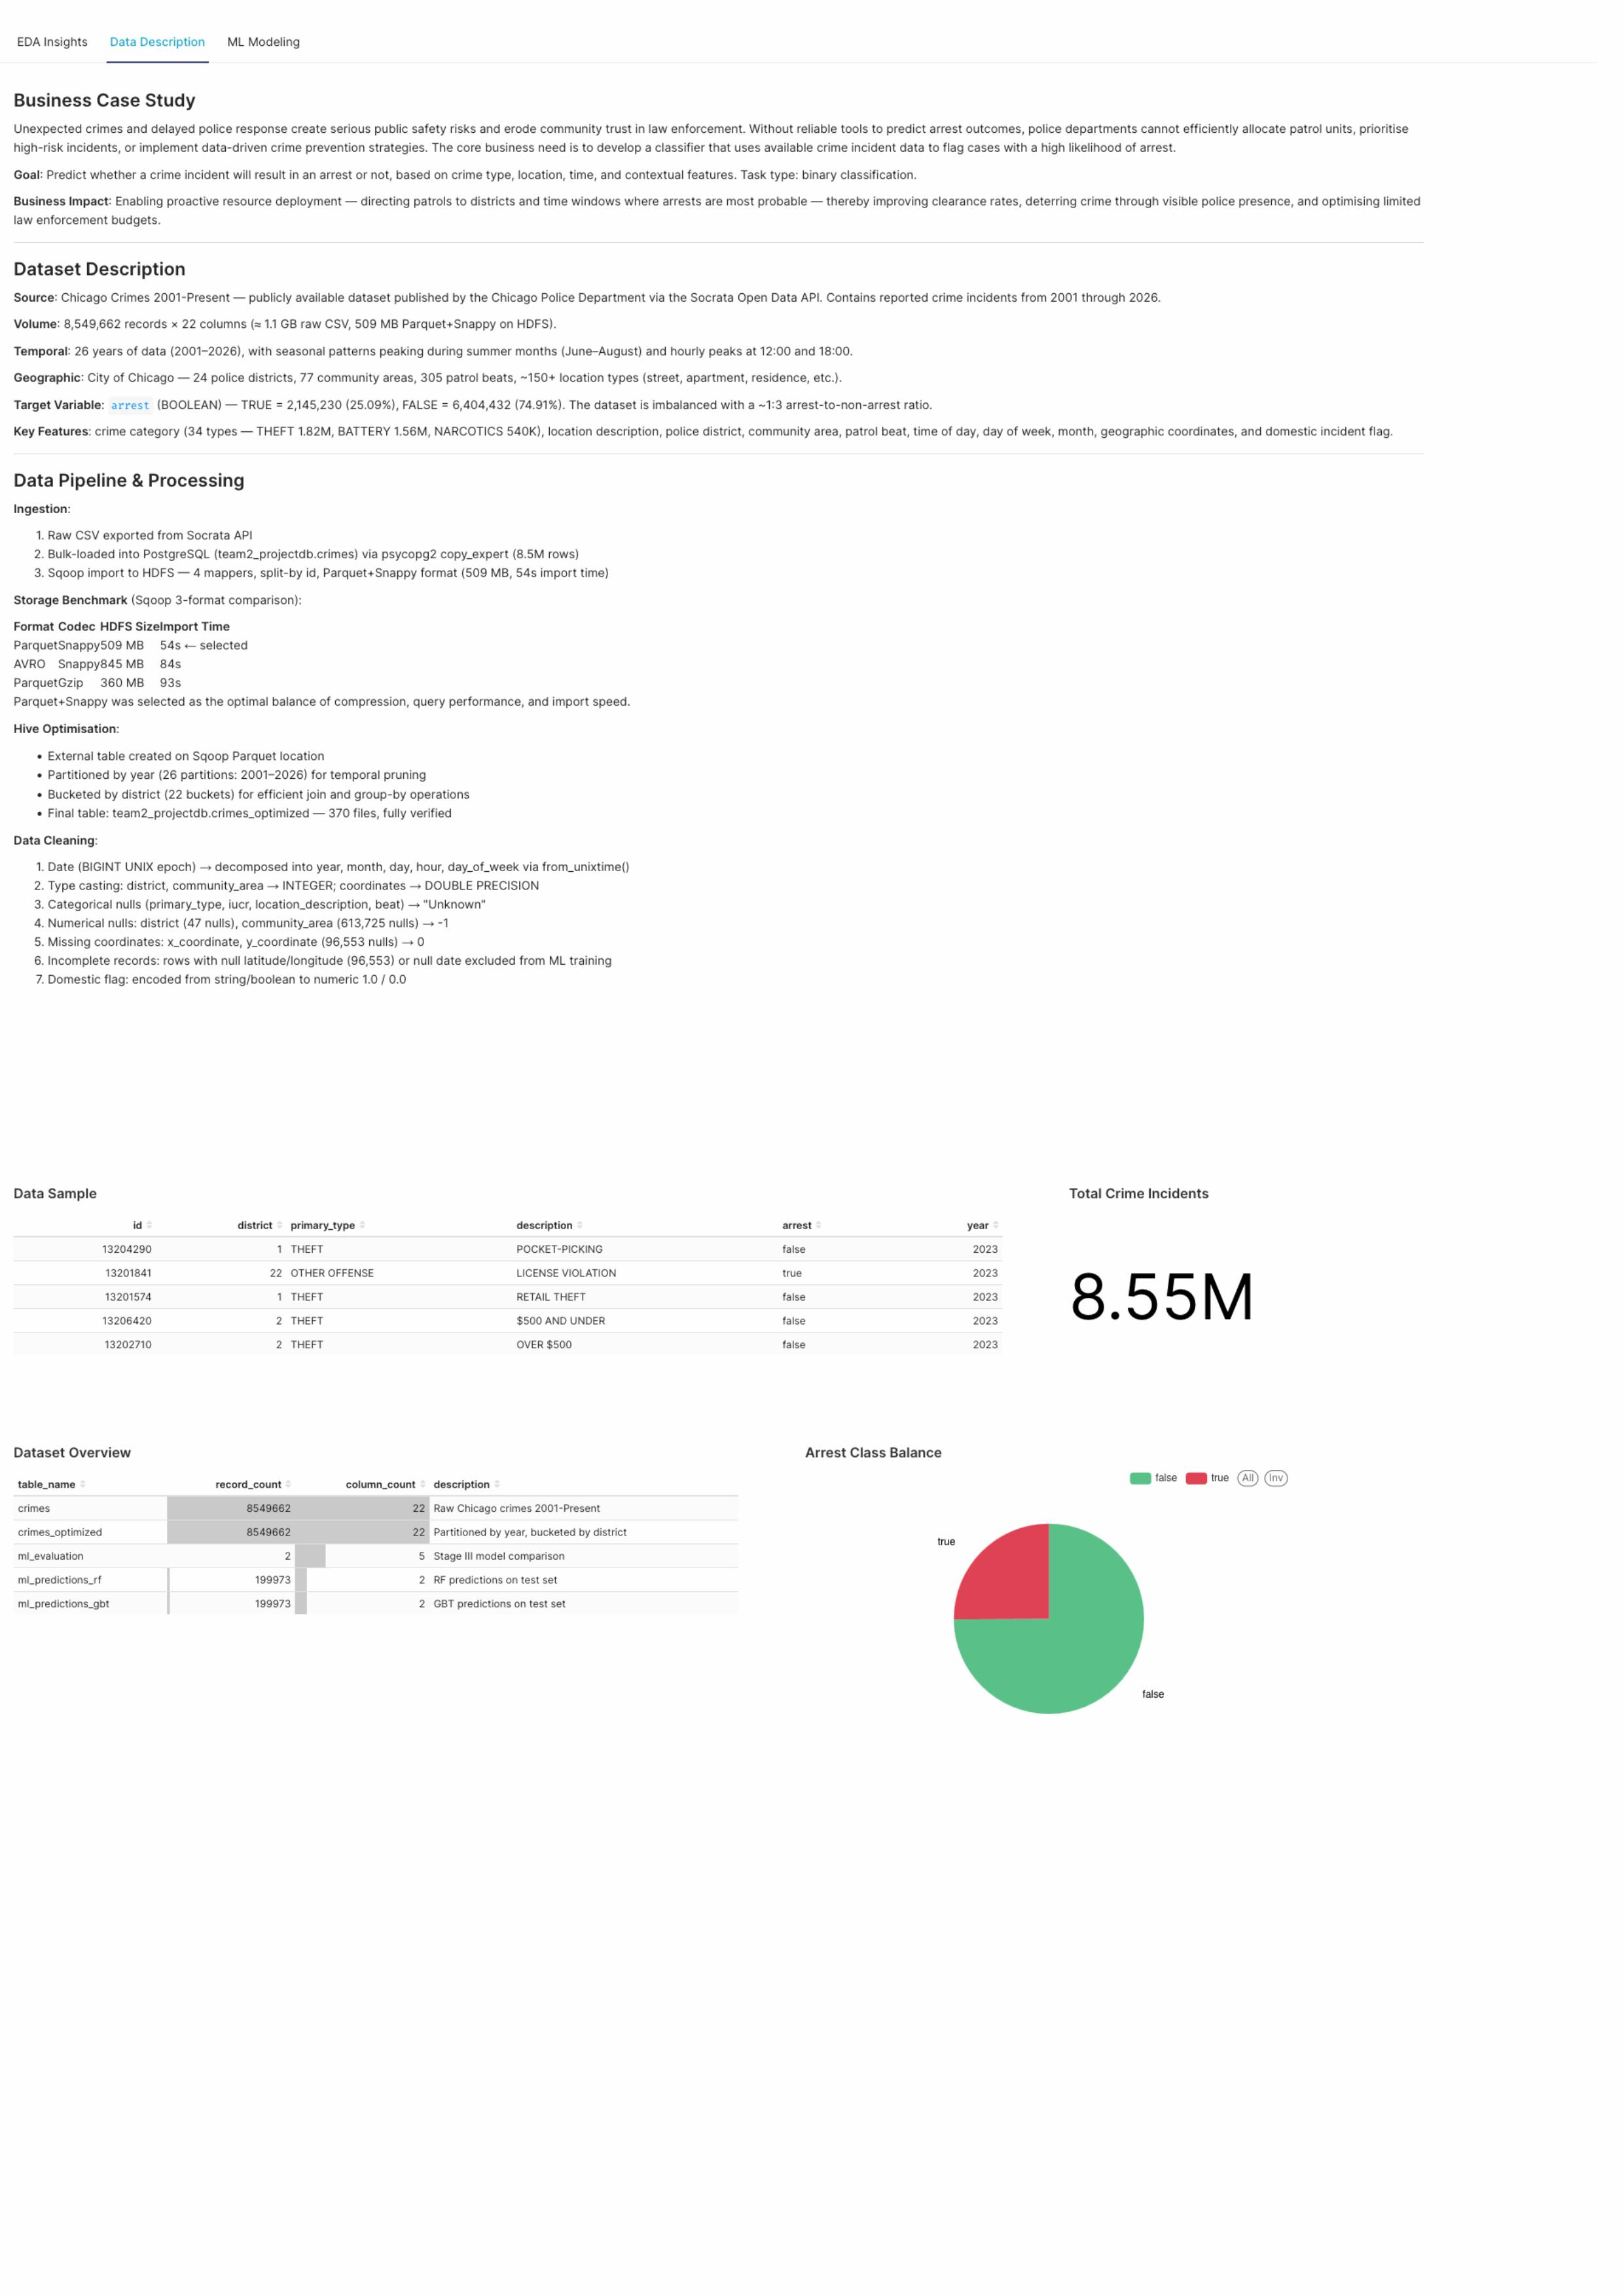
\includegraphics[width=0.85\textwidth]{output/dashboarddata1.jpg}
    \caption{Dashboard Tab 1: Data Description — dataset overview, schema, class balance, and data cleaning summary}
    \label{fig:dashboard-data1}
\end{figure}

\begin{figure}[H]
    \centering
    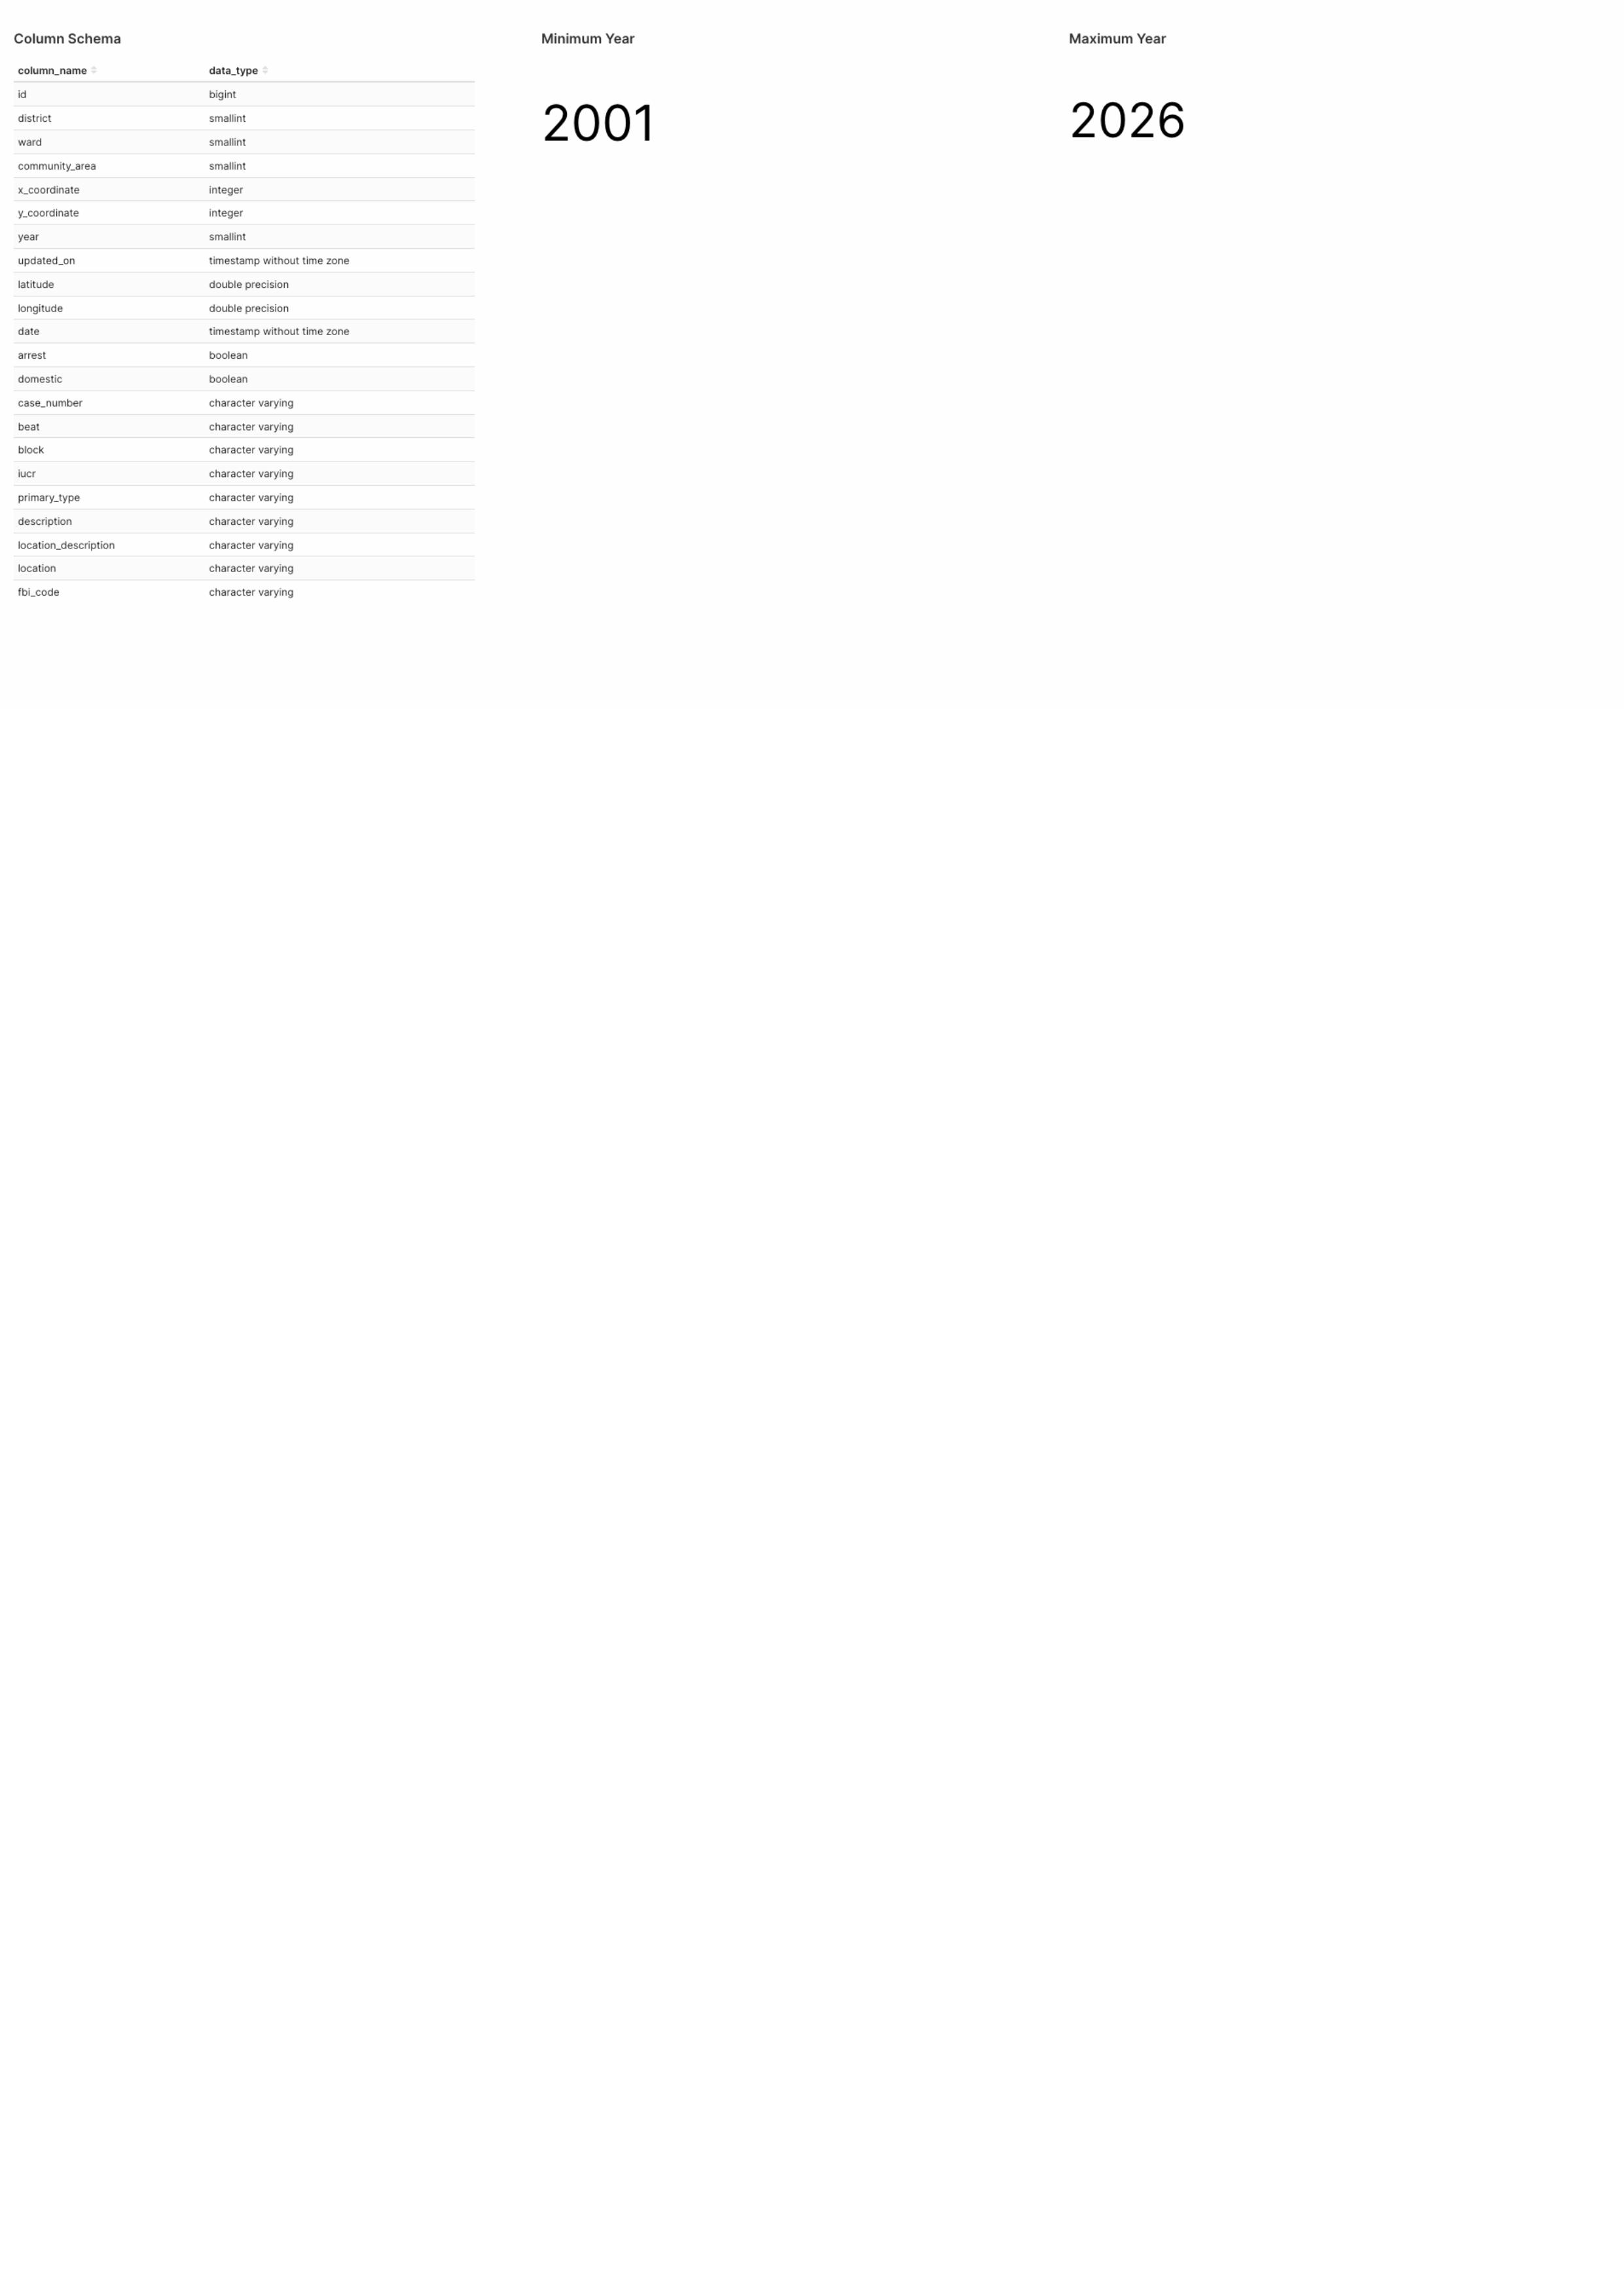
\includegraphics[width=0.85\textwidth]{output/dashboarddata2.jpg}
    \caption{Dashboard Tab 1: Data Description (continued) — year range and data cleaning text}
    \label{fig:dashboard-data2}
\end{figure}

\begin{figure}[H]
    \centering
    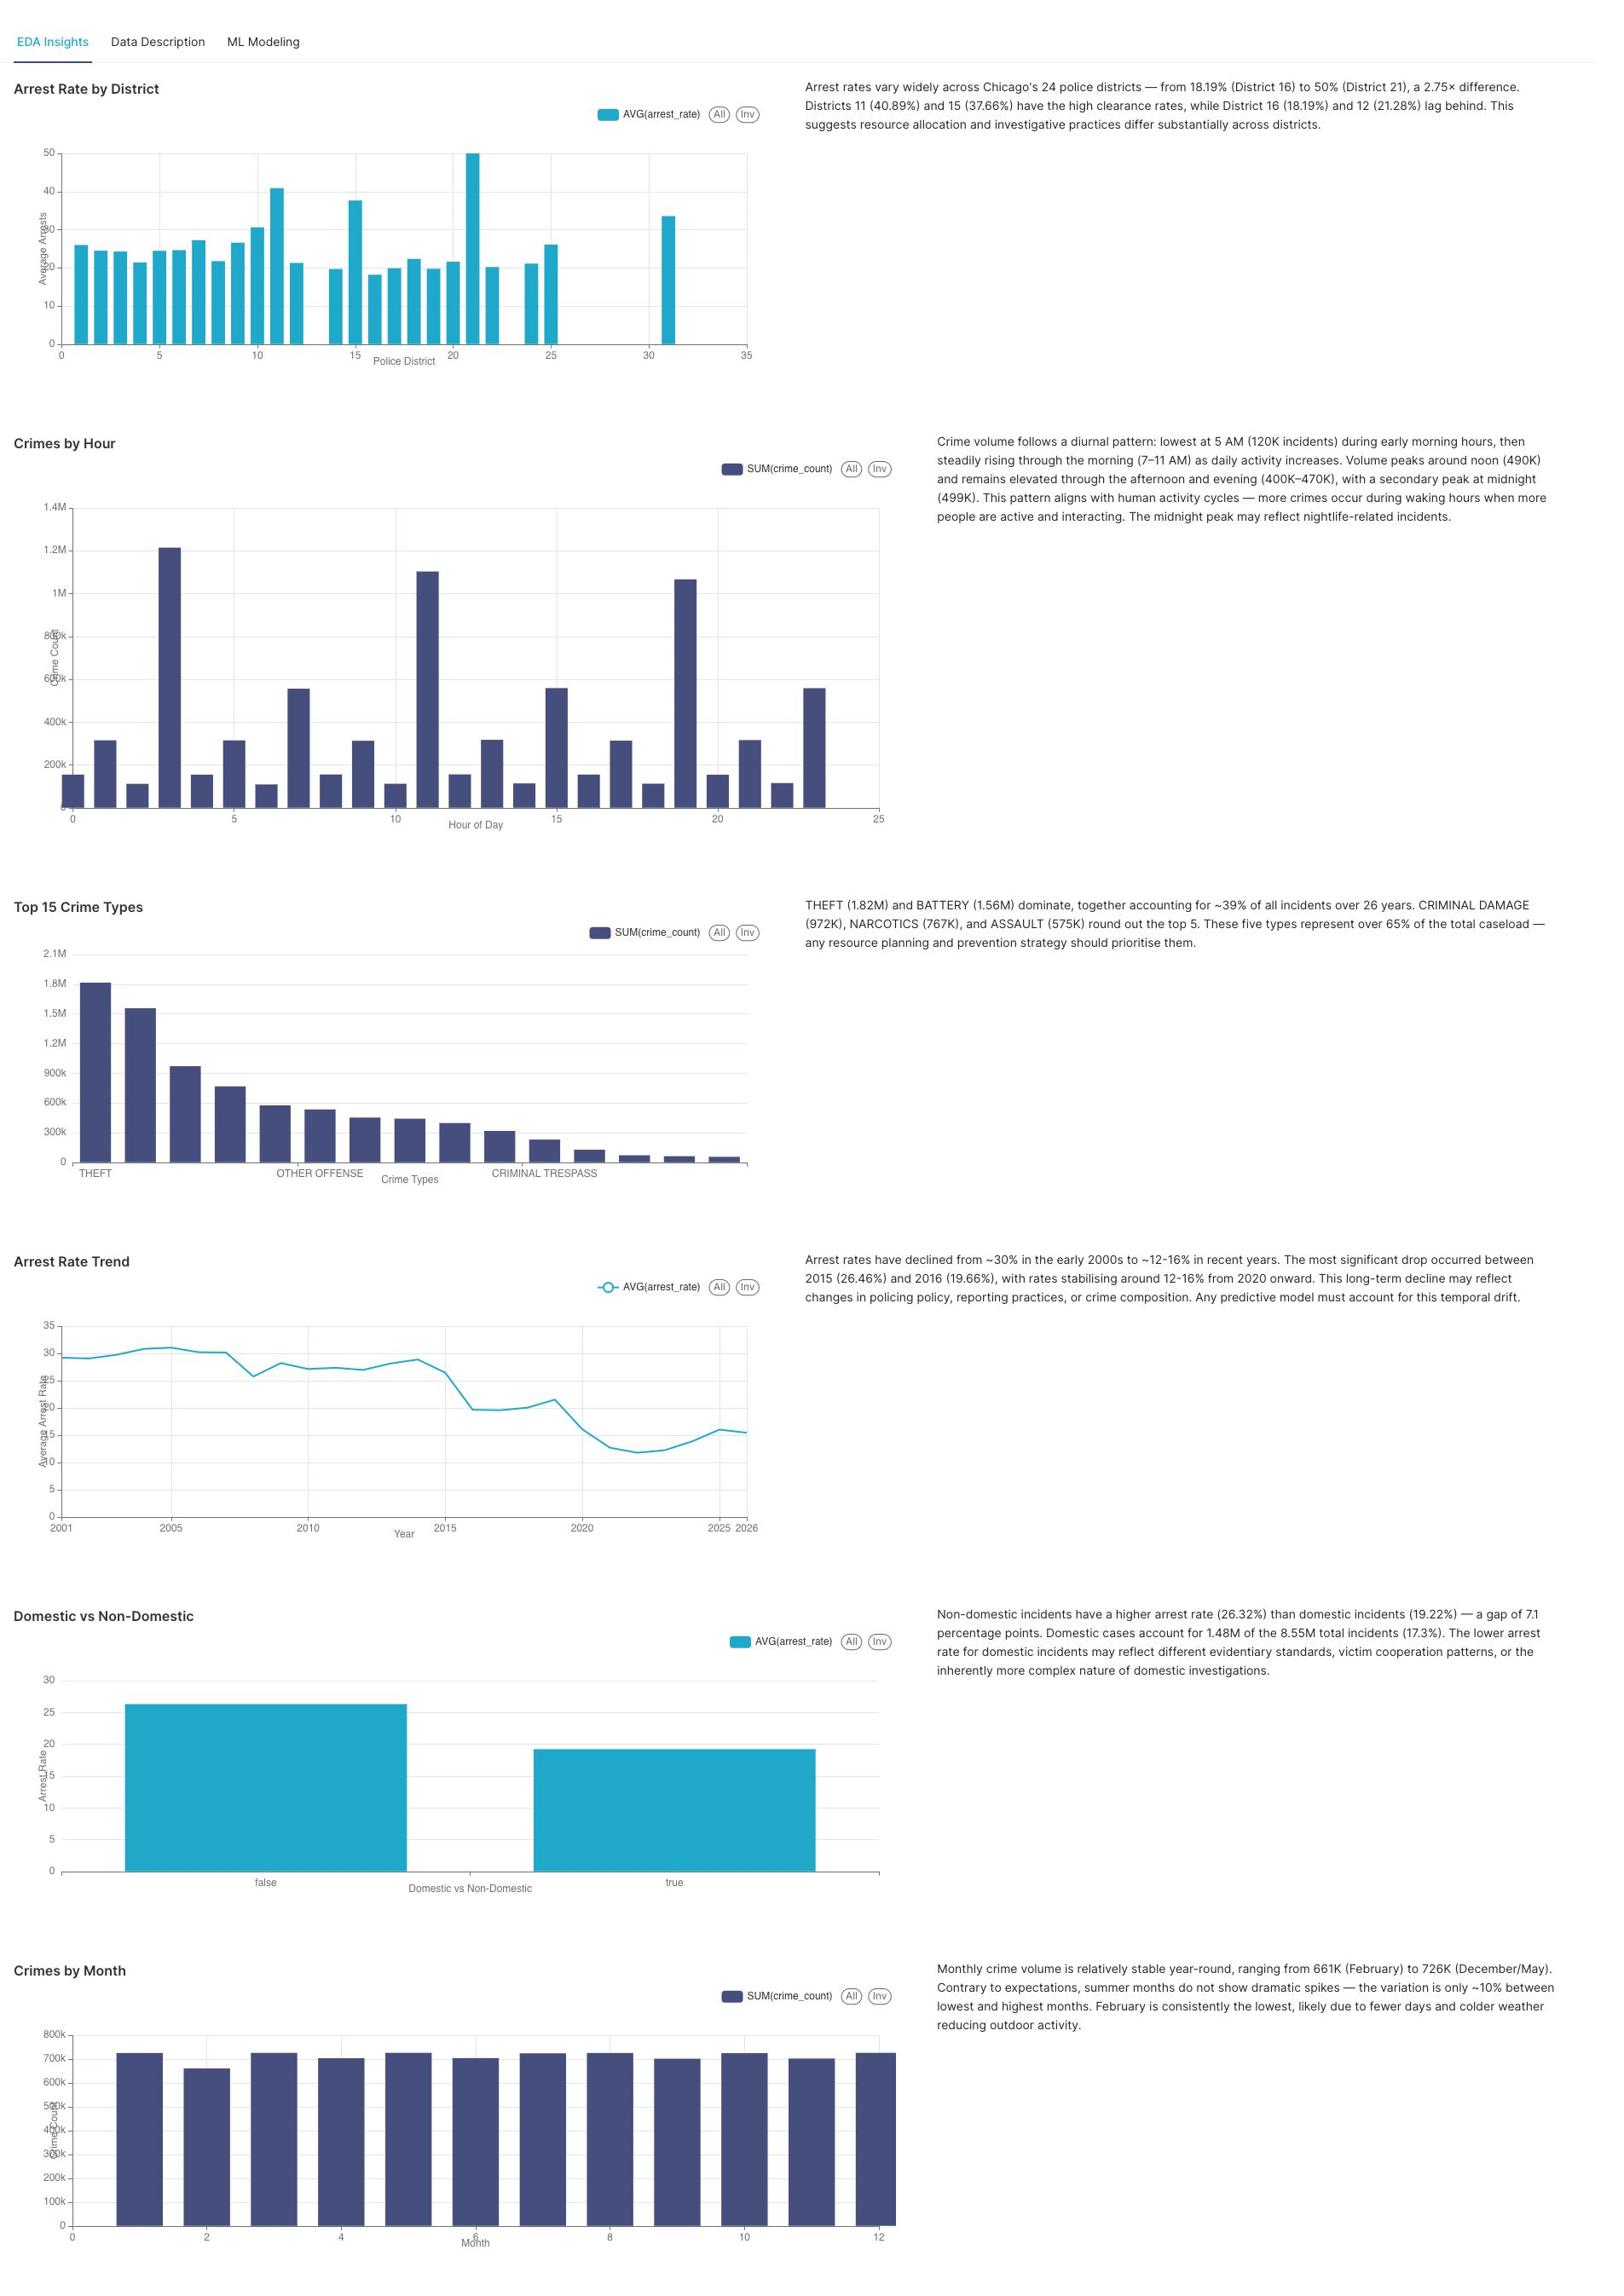
\includegraphics[width=0.85\textwidth]{output/dashboard_q1-q6.jpg}
    \caption{Dashboard Tab 2: EDA Insights — arrest rate by district, top crime types, crimes by hour, arrest rate trend, crimes by month, arrest by community area}
    \label{fig:dashboard-eda1}
\end{figure}

\begin{figure}[H]
    \centering
    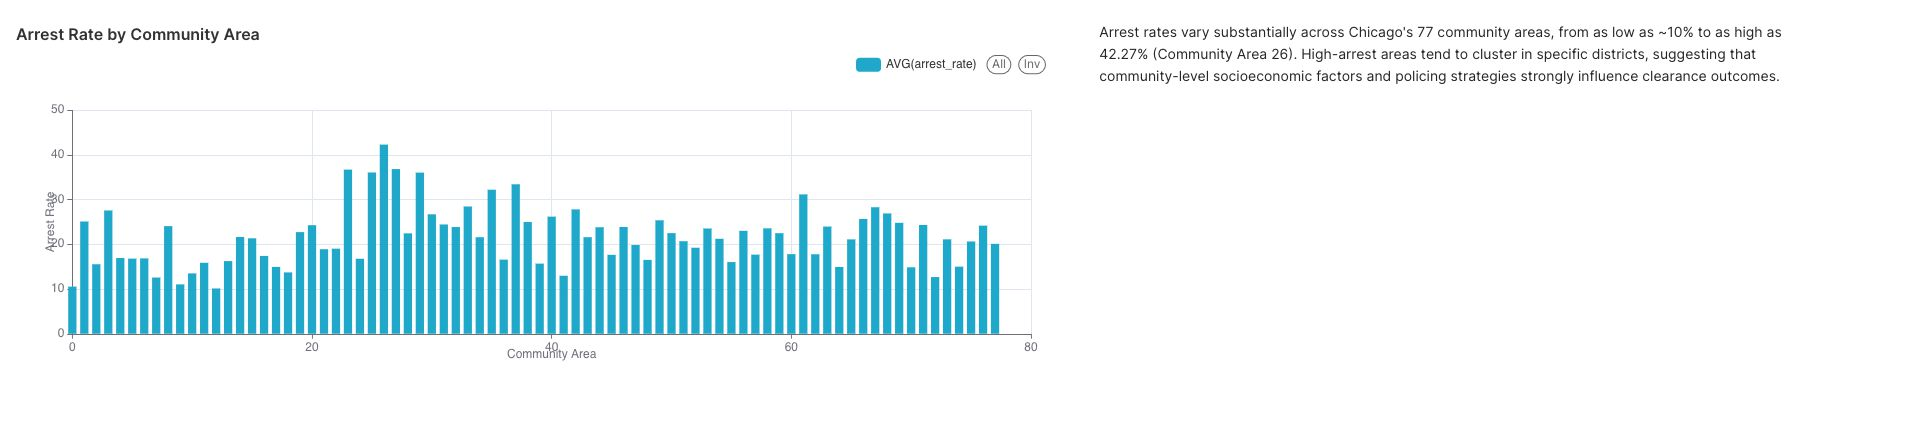
\includegraphics[width=0.85\textwidth]{output/dashboardq7.jpg}
    \caption{Dashboard Tab 2: EDA Insights (continued) — domestic vs non-domestic arrest rates}
    \label{fig:dashboard-eda2}
\end{figure}

\begin{figure}[H]
    \centering
    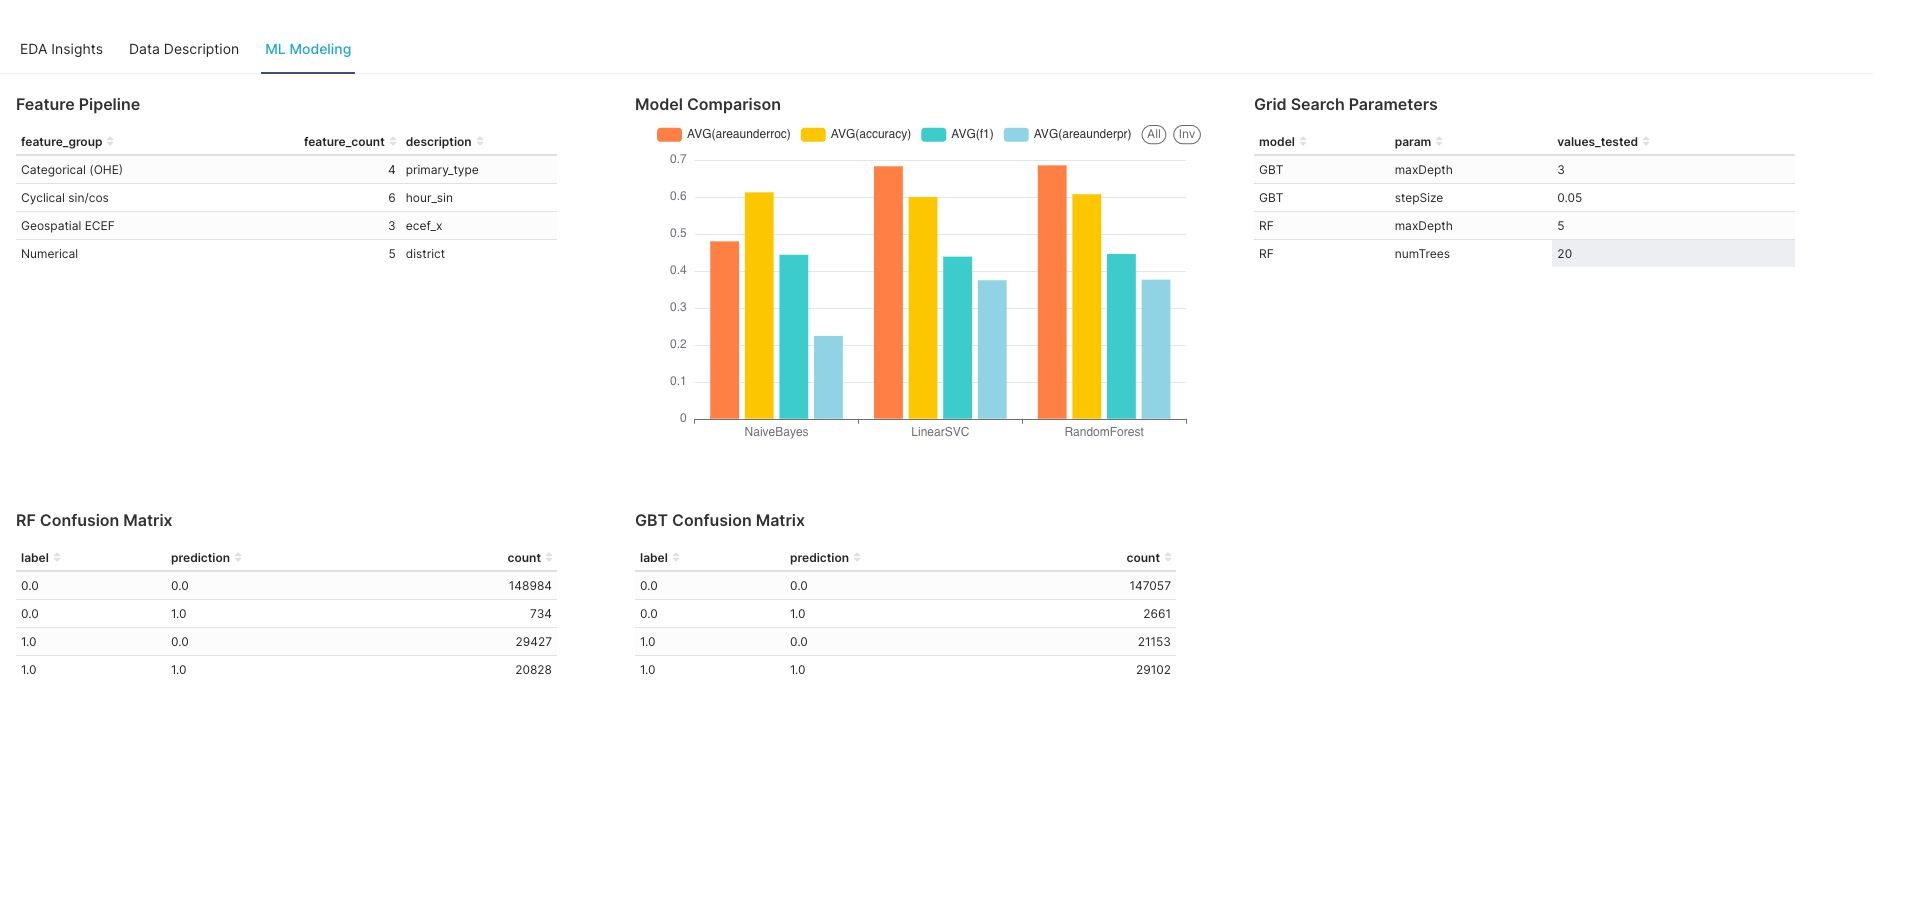
\includegraphics[width=0.85\textwidth]{output/mlDashboard.jpg}
    \caption{Dashboard Tab 3: ML Modeling — feature pipeline, grid search parameters, model comparison, and confusion matrices}
    \label{fig:dashboard-ml}
\end{figure}

\subsubsection{Stage II EDA Dashboard}

\begin{figure}[H]
    \centering
    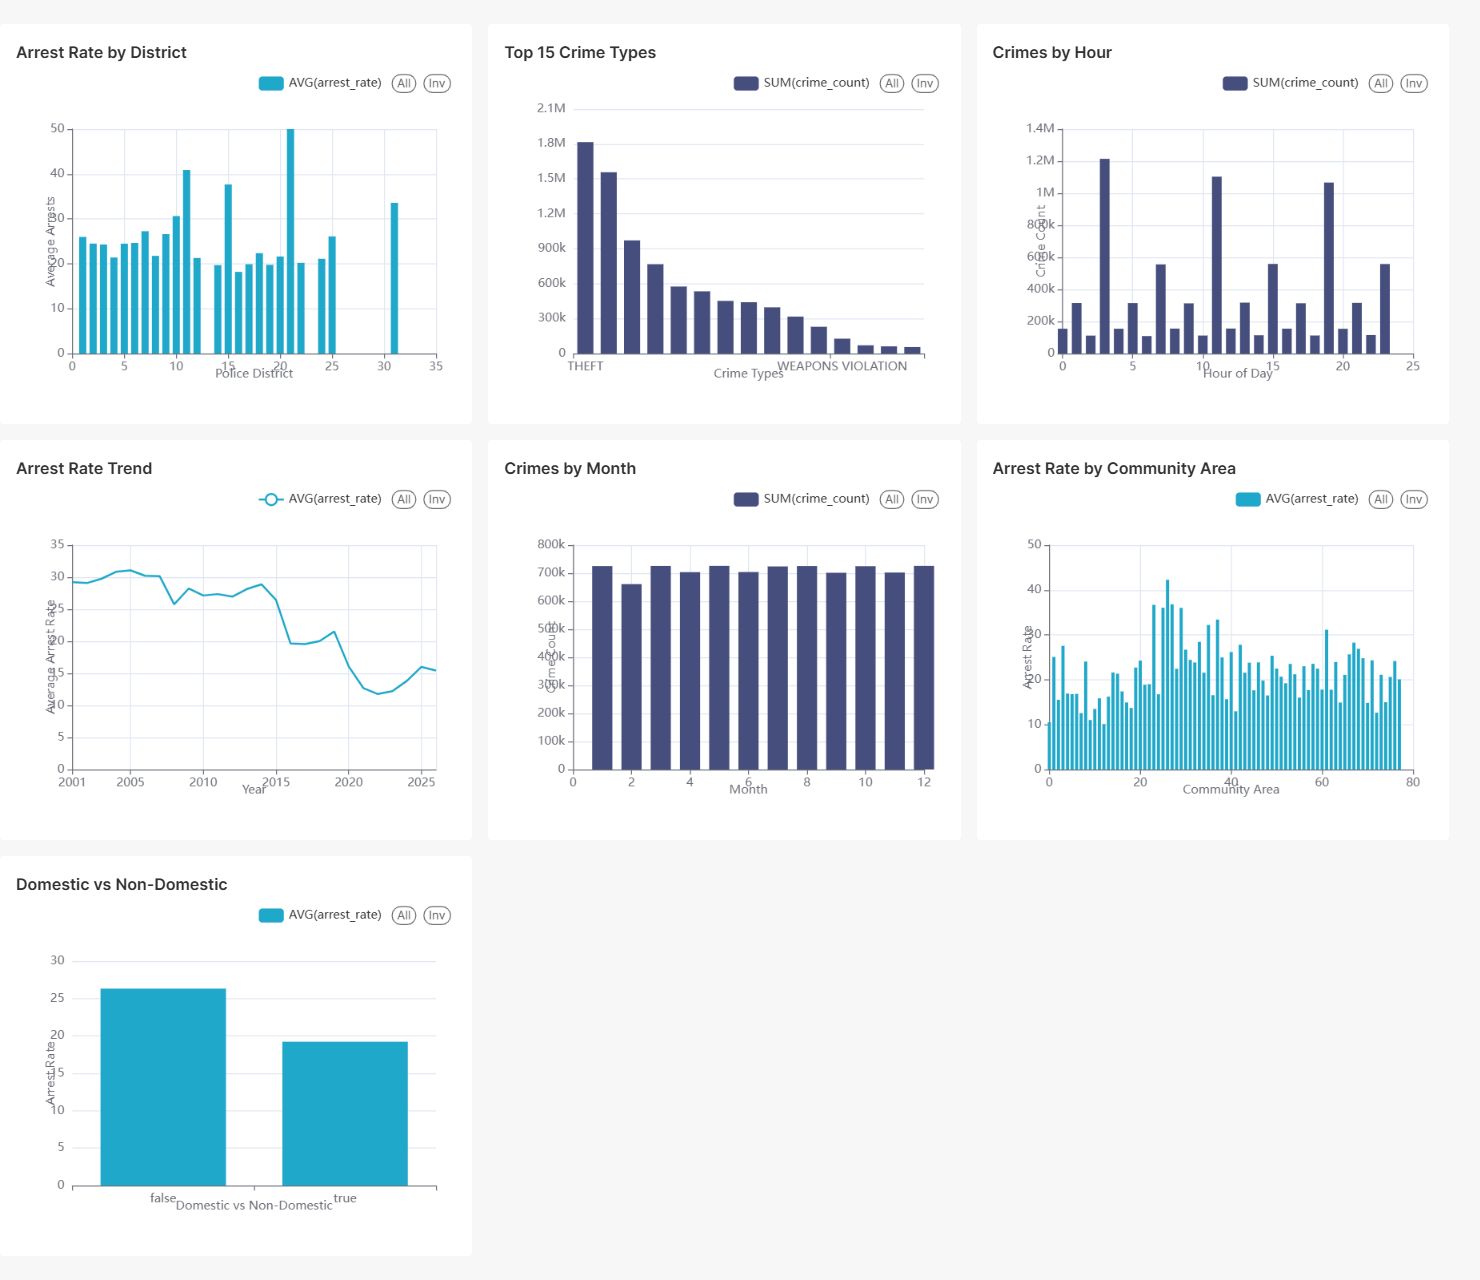
\includegraphics[width=0.9\textwidth]{output/dashboard.jpg}
    \caption{Stage II EDA Dashboard (initial 7 charts)}
    \label{fig:dashboard-stage2}
\end{figure}
